\chapter{Music}

\begin{definition}{Wave}{wave}
  A wave is something which moves back and forth over time. We will refer to
  waves as functions over time which output a number between in the range $
  \left[ -1,1 \right]$ where at rest it outputs $ 0$. In other words a wave is a
  periodic function: 
  \[
   w : [0, \infty) \to \left[ -1,1 \right] 
  \]
\end{definition}





Based on the definition of wave, it is clear that by creating a pressure wave that tranvels through the air which is an analog of the wave, then we can hear sound, we will call this a sound wave.

\begin{definition}{Note}{note}
  Given a musical system, a note is a pitch which can be generated from the
  system.
\end{definition}

\begin{definition}{Wave Quality}{wave_quality}
  Two waves $ w\left(t\right), v\left(t\right)$ are said to have the same quality when there is an $ \alpha \in \mathbb{R}$ such that for any $ t \in [0, \infty)$ 
  \[
  w\left(t\right) =  v\left(\alpha t\right)
  \]
  In other words, they only differ by a scaling in the $x$ direction, that is to say, their wave shape is the same. 

\end{definition}

\begin{proposition}{Sine with Different Frequencies have the same Wave
Quality}{sine_with_different_frequencies_have_the_same_wave_quality}
    Any two waves given by \( \sin  \left( \alpha x \right) \) , \( \sin
    \left( \beta x \right) \) for \( \alpha , \beta  \in \mathbb{R} ^{ \neq 0 }
    \) have the same wave quality.
\end{proposition}
\begin{proof}
    Visually we can first see that:
    \begin{center}
        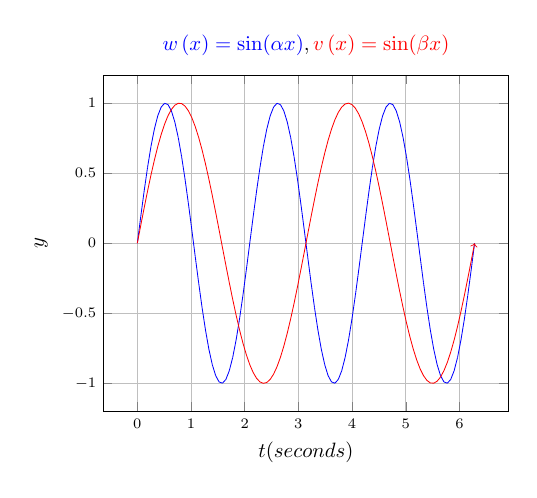
\begin{tikzpicture}[scale=.75]
          \begin{axis} [
              title = {$\textcolor{blue}{  w\left(x\right) = \sin(\alpha x)},
              \textcolor{red}{v\left(x\right) = \sin(\beta x)}$},
              xtick = {0,...,2 * pi},
              xlabel = $t (\text{seconds})$, ylabel = $y$,
              ticklabel style = {font = \scriptsize},
              grid
            ]
            \addplot [->, surf, domain=0:2 * pi , samples=100,blue, thin] { sin(3 * deg(x) ) };
            \addplot [->, domain=0:2 * pi , samples=100,red, thin] { sin(2 * deg(x) ) };
          \end{axis}
        \end{tikzpicture}
    \end{center}

    It's clear that one is a compression of the other, formally we can see that
    the red wave's period can be scaled by \( \frac{\alpha }{\beta } \) to
    become the blue wave.

  Notice that given a wave, and $ k \in \mathbb{R} ^{> 1}$ that $ u\left(kx\right)$ becomes compressed, and thus has a higher pitch.
\end{proof}


In general we will measure the period of all waves in seconds, for example the red wave in the previous definition has a period of $ \pi$ seconds. We are measuring this in seconds so we can start moving more towards the system we would like to discuss, which uses the unit $ \text{Hz}$, which is a way to measure frequency.

\begin{definition}{Frequency}{frequency}
  Frequency is the number of occurances of an event in a determined time interval. In terms of waves, we recall that the period of a wave is the amount of time for one cycle to complete, therefore the frequency of the cycles should be $\frac{1}{P}$, that is, after $ P$ time units $ 1$ cycle has finished.

  Remark: Since we think of waves abstractly as sine waves, the only thing that differentiates them is their frequency, therefore we may use the frequency of a wave rather than talk about the wave itsefl in dicsussion.
\end{definition}

Since we have chosen a time unit of seconds, we would now be able to say that the frequency of the red wave is $ \frac{1}{\pi}$ cycles per second. The unit $ \text{Hz}$ specifies occurances per second, so we could say that the red wave has a frequency of $ \frac{1}{\pi} \text{Hz}$ 


The reason why we have gone through all of these definitions is so we can grapple with the system of equal temperament. The system of equal temperament is an approximation of another pitch generating system called just intonation, one might ask: "If it's just an approximation, then why not just use just intonation?". Equal temperatment brings some new things to the table, it allows us to take two notes that are a certain distance apart, move them both up an equal distance and when these new notes are played together it produces a wave of the same quality.

We will come back to this interesting property of the equal temperament system after we get some more preliminaires. After we fully understand what it is trying to approximate

\section{Just Intonation}

Just intonation constructs it's notes by using ratios with respect to some base frequency. For example let's start with a tone with some frequency $x\text{Hz}$, and call it the note C, let's now produce a new frequency which is higher so that every time that the frequency (thinking of a frequency as a wave) of C completes two cycles, this new frequency completes three.  When this is the case we will say that this new note is in ratio $2:3$ with C, and we will call this note G.

When these two notes are played simultaneously (say on a piano), we can realize that when the two notes are played, two different strings vibrate, and as those waves travel through the air as pressure waves, they will combine with eachother,  so if the trough of one wave lines up with the peak of the other, we should get some sort of cancellation, to combine them in our model of waves we can analgously add the two waves values together. We can simply think of this summation as a single wave that travels into our ears.

Due to this we can now think of C being played with the new note, and consider that a new wave. Let's visualize C and G being played together.

\begin{center}
  % \pgfplotsset{width=\linewidth * 3/4}
  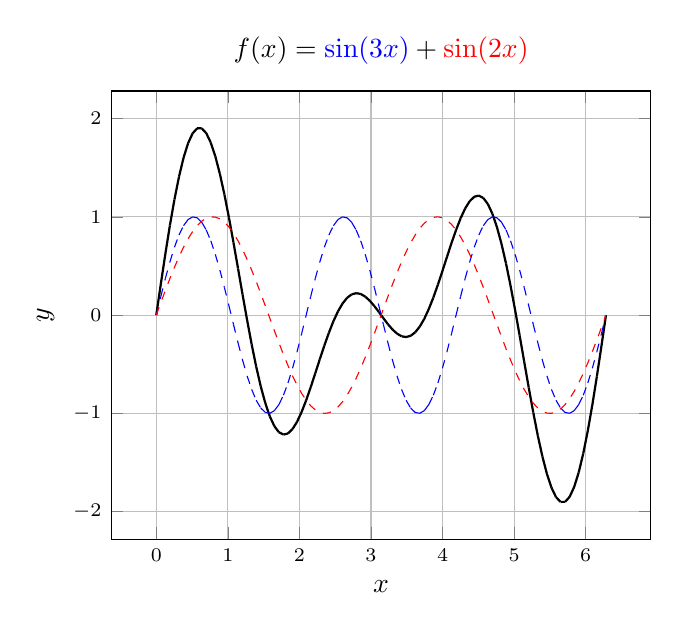
\begin{tikzpicture}
    \begin{axis} [
      title = {$f(x) = \textcolor{blue}{\sin(3x)} + \textcolor{red}{\sin(2x)}$},
      xtick = {0,...,2 * pi},
      xlabel = $x$, ylabel = $y$,
      ticklabel style = {font = \scriptsize},
      grid
      ]
      \addplot [->, surf, domain=0:2 * pi , samples=100, black, thick] { sin(3 * deg(x) ) + sin(2 * deg(x)) };
      \addplot [ surf, domain=0:2 * pi , samples=100,blue, thin, dashed] { sin(3 * deg(x) ) };
      \addplot [domain=0:2 * pi , samples=100,red, thin, dashed] { sin(2 * deg(x) ) };
    \end{axis}
  \end{tikzpicture}
\end{center}
              


For example let's compare our previous ratio of $2:3$ with a ratio of $2: 7$ 

\begin{center}
  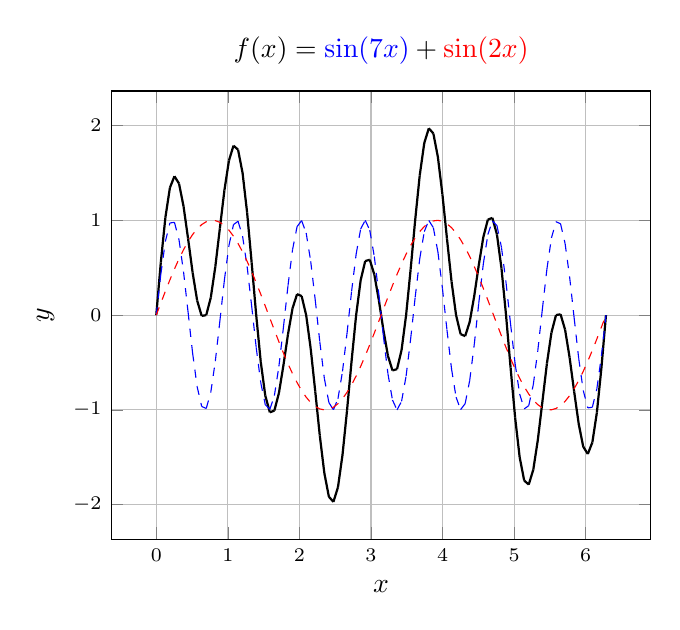
\begin{tikzpicture}
    \begin{axis} [
      title = {$f(x) = \textcolor{blue}{\sin(7x)} + \textcolor{red}{\sin(2x)}$},
      xtick = {0,...,2 * pi},
      xlabel = $x$, ylabel = $y$,
      ticklabel style = {font = \scriptsize},
      grid
      ]
      \addplot [->, surf, domain=0:2 * pi , samples=100, black, thick] { sin(7 * deg(x) ) + sin(2 * deg(x)) };
      \addplot [ surf, domain=0:2 * pi , samples=100,blue, thin, dashed] { sin(7 * deg(x) ) };
      \addplot [domain=0:2 * pi , samples=100,red, thin, dashed] { sin(2 * deg(x) ) };
    \end{axis}
  \end{tikzpicture}
\end{center}
              

We can visually see the that the 2:3 ratio is less complex, go to my website and find the recording of each, and compare their complexity, for me there seems to be a connection between complexity and how harmonious these ratios are. For example if we consider the following sounds 2:3, 2:5, 2:7, 2:9, 2:11, and so on, we notice that visually it becomes more complex and also the interval sounds more complex.

Now continuing with the other ratios that were chosen for just intonation, we get the following:

[Table of the different just intonantion ratios]

Here let's sort the following intervals by their complexity and then listen to them in order

Based on this table we have generated 12 new tones and we can lable them as follows. In this musical system we don't restrict ourselves to these tones only, but also multiples or divisions of two of these notes. And they get labelled by the same letter. This starts the whole cyclic way of thinking

\begin{definition}{Exponent}{exponent}
  For any $ b \in \mathbb{R}, n \in \mathbb{Z}$ we have
  \[
    b ^{n} \stackrel{\mathtt{D}}{=} \underbrace{b  \cdot b \dotsb b  \cdot b}_{n \text{times}}
  \]
  Note: The definition can be extended for $ n \in \mathbb{R}$ but four our purposes, this will do
\end{definition}

It does so by first having some base frequency and then producing all other notes based on that frequency. A common choice for this frequency is $440\text{Hz}$. The method for producing new notes is by taking a frequency that is already part of the system and multiplying it's frequency by $2^(\frac{1}{12})$ or $2^(\frac{-1}{12})$. The choice of $2^(\frac{\pm1}{12})$ may not make any sense right now, so to make it make sense, we will develop our understanding of the just intonation system.


The reason why we allow multiples of two of these notes is that it doesn't change the quality of the notes, listen to the pitch 440, and the pitch 880, they should have the same quality, but one sounds higher than the other. This is what allous the system to have some many notes, in fact both of these musical systems have infintiely many notes, but us as humans can only hear within a certain range, so we can only perceive a subset of these notes.

So now back to understanding the choice of $2^12$. Consider just intonation with all of it's notes, if we take C, then the note which is seven notes higher is in ratio $2:3$ with C, in equal temperament if we want a note which is 7 notes higher, then we are multiplying by $2^(\frac{1}{12})$ seven times in a row which is the same as multiplying by $2^(\frac{7}{12})$ one time which is approximately equal to $1.498$, that's awfully close to $1.5$, that means that this new pitch is oscillating 1.5 times faster than the original pitch, this also means that in the time that the first pitch complestes 2 cycles, the other pitch will have completed $2 * 1.5 = 2 + 1 = 3$ cycles, therefore we can see that these two pitches are approximately in the ratio $2:3$. If we do the same analysis for each of the other numbers ($2^(k/12)$ for $k = 0, ..., 11$, you see that each time it correctly approximates the ratio), notice that when k is a multiple of 12 that you get $2^m$ for some integer $m$. Because of this it means that multiplying by $2^m$ just gives us the same note in a different octave.

Due to the above we have some motativation for some notation, we will first consider the note C somewhere in equal temperament, to get the note which is one note higher than it we multiply by $2^(\frac{1}{12})$, to get the note which is 2 higher than it we multiply by $2^(\frac{2}{12})$ and so on, therefore we will associate these numbers with the notes themselves, also notice that when we multiply C's pitch by $2^(\frac{0}{12}) = 1$ you end with C again, so we will write $0^{\star}$ for C, $1^{\star}$ for C\#/Db,  and so on.

We will also associate the gap between any two consecutive notes as a semitone. So if you start at B and go down two semitones you get to A, in the new notation, that would be saying that if you start at $11^{\star}$ and you go down two semitones that you arrive at $9^{\star}$.

So now with all this newly aquired information we are ready to understand our original proposition in greater detail, the proposition that I am referring two is 

"two notes that are a certain distance apart, move them both up an equal number of notes and when these new notes are played together it produces the same quality."

or reformulated, any two notes which are n semitones away have the same quality.

To understand why all we have to do is remember that in equal temperament a note that is n semitones away is just the lower note multiplied by $2^(\frac{n}{12})$ (or the higher divided by $2^(\frac{n}{12})$). Therefore because of https://www.desmos.com/calculator/5km4qgfom5 the quality is the same.

So far we have been talking about moving notes up, and adding semitones to notes, right now we will formally define what that means.

If you are at C and you add 7 semitones to that note you end up at a G, in the standard system you would just have to count up the letter names. When you are using our system it becomes clear, $0^{\star} + 7 = 7^{\star}$, so in general we get the following definition.

Definition: Adding a number to a note

\begin{definition}{Semitone Integer Notation}{semitone_integer_notation}
  \begin{itemize}
    \item For any $\alpha \in \mathbb{Z}$
      \[
        x^{\star}  +  \alpha \stackrel{\mathtt{D}}{=} \left( x  +  \alpha \right)^{\star}
      \]
  \end{itemize}
  \subsubsection*{Examples}
  \begin{itemize}
    \item If $x = 5$ and $\alpha = 9$
      \[
        5^{\star}  +  9 = 14^{\star} = 2^{\star}
      \] 
    \item $x = 9$ $\alpha = -14$ 
      \[
        9^{\star}  +   - 14 = 9  -  14^{\star} =   - 5^{\star} = 7^{\star}
      \]
  \end{itemize}
\end{definition}

Therefore for any two notes we can always add a certain number of semitones to the note to get to the other, formally we have

\begin{definition}{Musical Interval}{musical_interval}
    The interval from  $ x^{\star}$ to $ y ^{\star}$ (where $ x^{\star}, y^{\star} \in \mathbb{W}$) is the number of semitones you have to add to $ x^{\star}$ to get to $ y^{\star}$, due to the interaction between NIN and SIN it follows that 
  \[
  x^{\star}  +  \left( y  -  x \right) = x  +  y  -  x^{\star} = y^{\star}
  \]
  Therefore in general the interval from $ x^{\star}$  to $ y^{\star}$ is $y  - x$ . And we define 
  \[
  I\left( x^{\star}, y^{\star}\right) \stackrel{\mathtt{D}}{=} (y  -  x) ~\%~ 12
  \]
  \subsubsection*{Examples}
  \begin{itemize}
    \item $I\left( 4^{\star}, 9^{\star}\right) = 9  -  4 = 5$ 
  \end{itemize}
\end{definition}

For any note we know that it is just is just a scaling of 440Hz, and therefore has the same quality as a single 440Hz pitch. Thus we should never focus on single notes, as individually they all have the same quality, if a series of notes are played over time, such that no two notes are ever played simultaneously then, we should look at these notes with respec to some base frequency so that we can analyze their quality or we could look at the relative intervals between consecutive notes so that we can analyze their quality in this way.

As of right now our notation doesn't specify an octave when we talk about notes, so to specify that we give an offset from C4 (frequency of that), and label that as 0, and for any number of octaves higher we add a number of ['] which will define how many octaves higher it is than the 4-th band, also we will use [,] to specify octaves lower, so that when we write 3'' we wwould be talking about 3 + (2)*12. and if we had 9,,,= 9 - (3)*12.
